We have made several attempts to adapt existing mechanisms into our model.
\subsection{DNA on Connected Network}
One of the outstanding works on double auctions on social networks is Double Network Auction (DNA)\cite{DNA}. The method is an extension of McAfee's trade reduction mechanism
that runs on several disjoint buyer networks. Therefore, we may reduce our model to DNA's model
by dividing the connected buyer networks into several disjoint smaller buyer networks according to the allocation
given by McAfee's method.
However, we can find a situation where the network is individable. Fig \ref*{fig:DNACounter}
shows one of the situations when several sellers together are connected to a chain of buyers. Therefore,
our problem setting cannot be reduced.
\begin{figure}[htbp]
  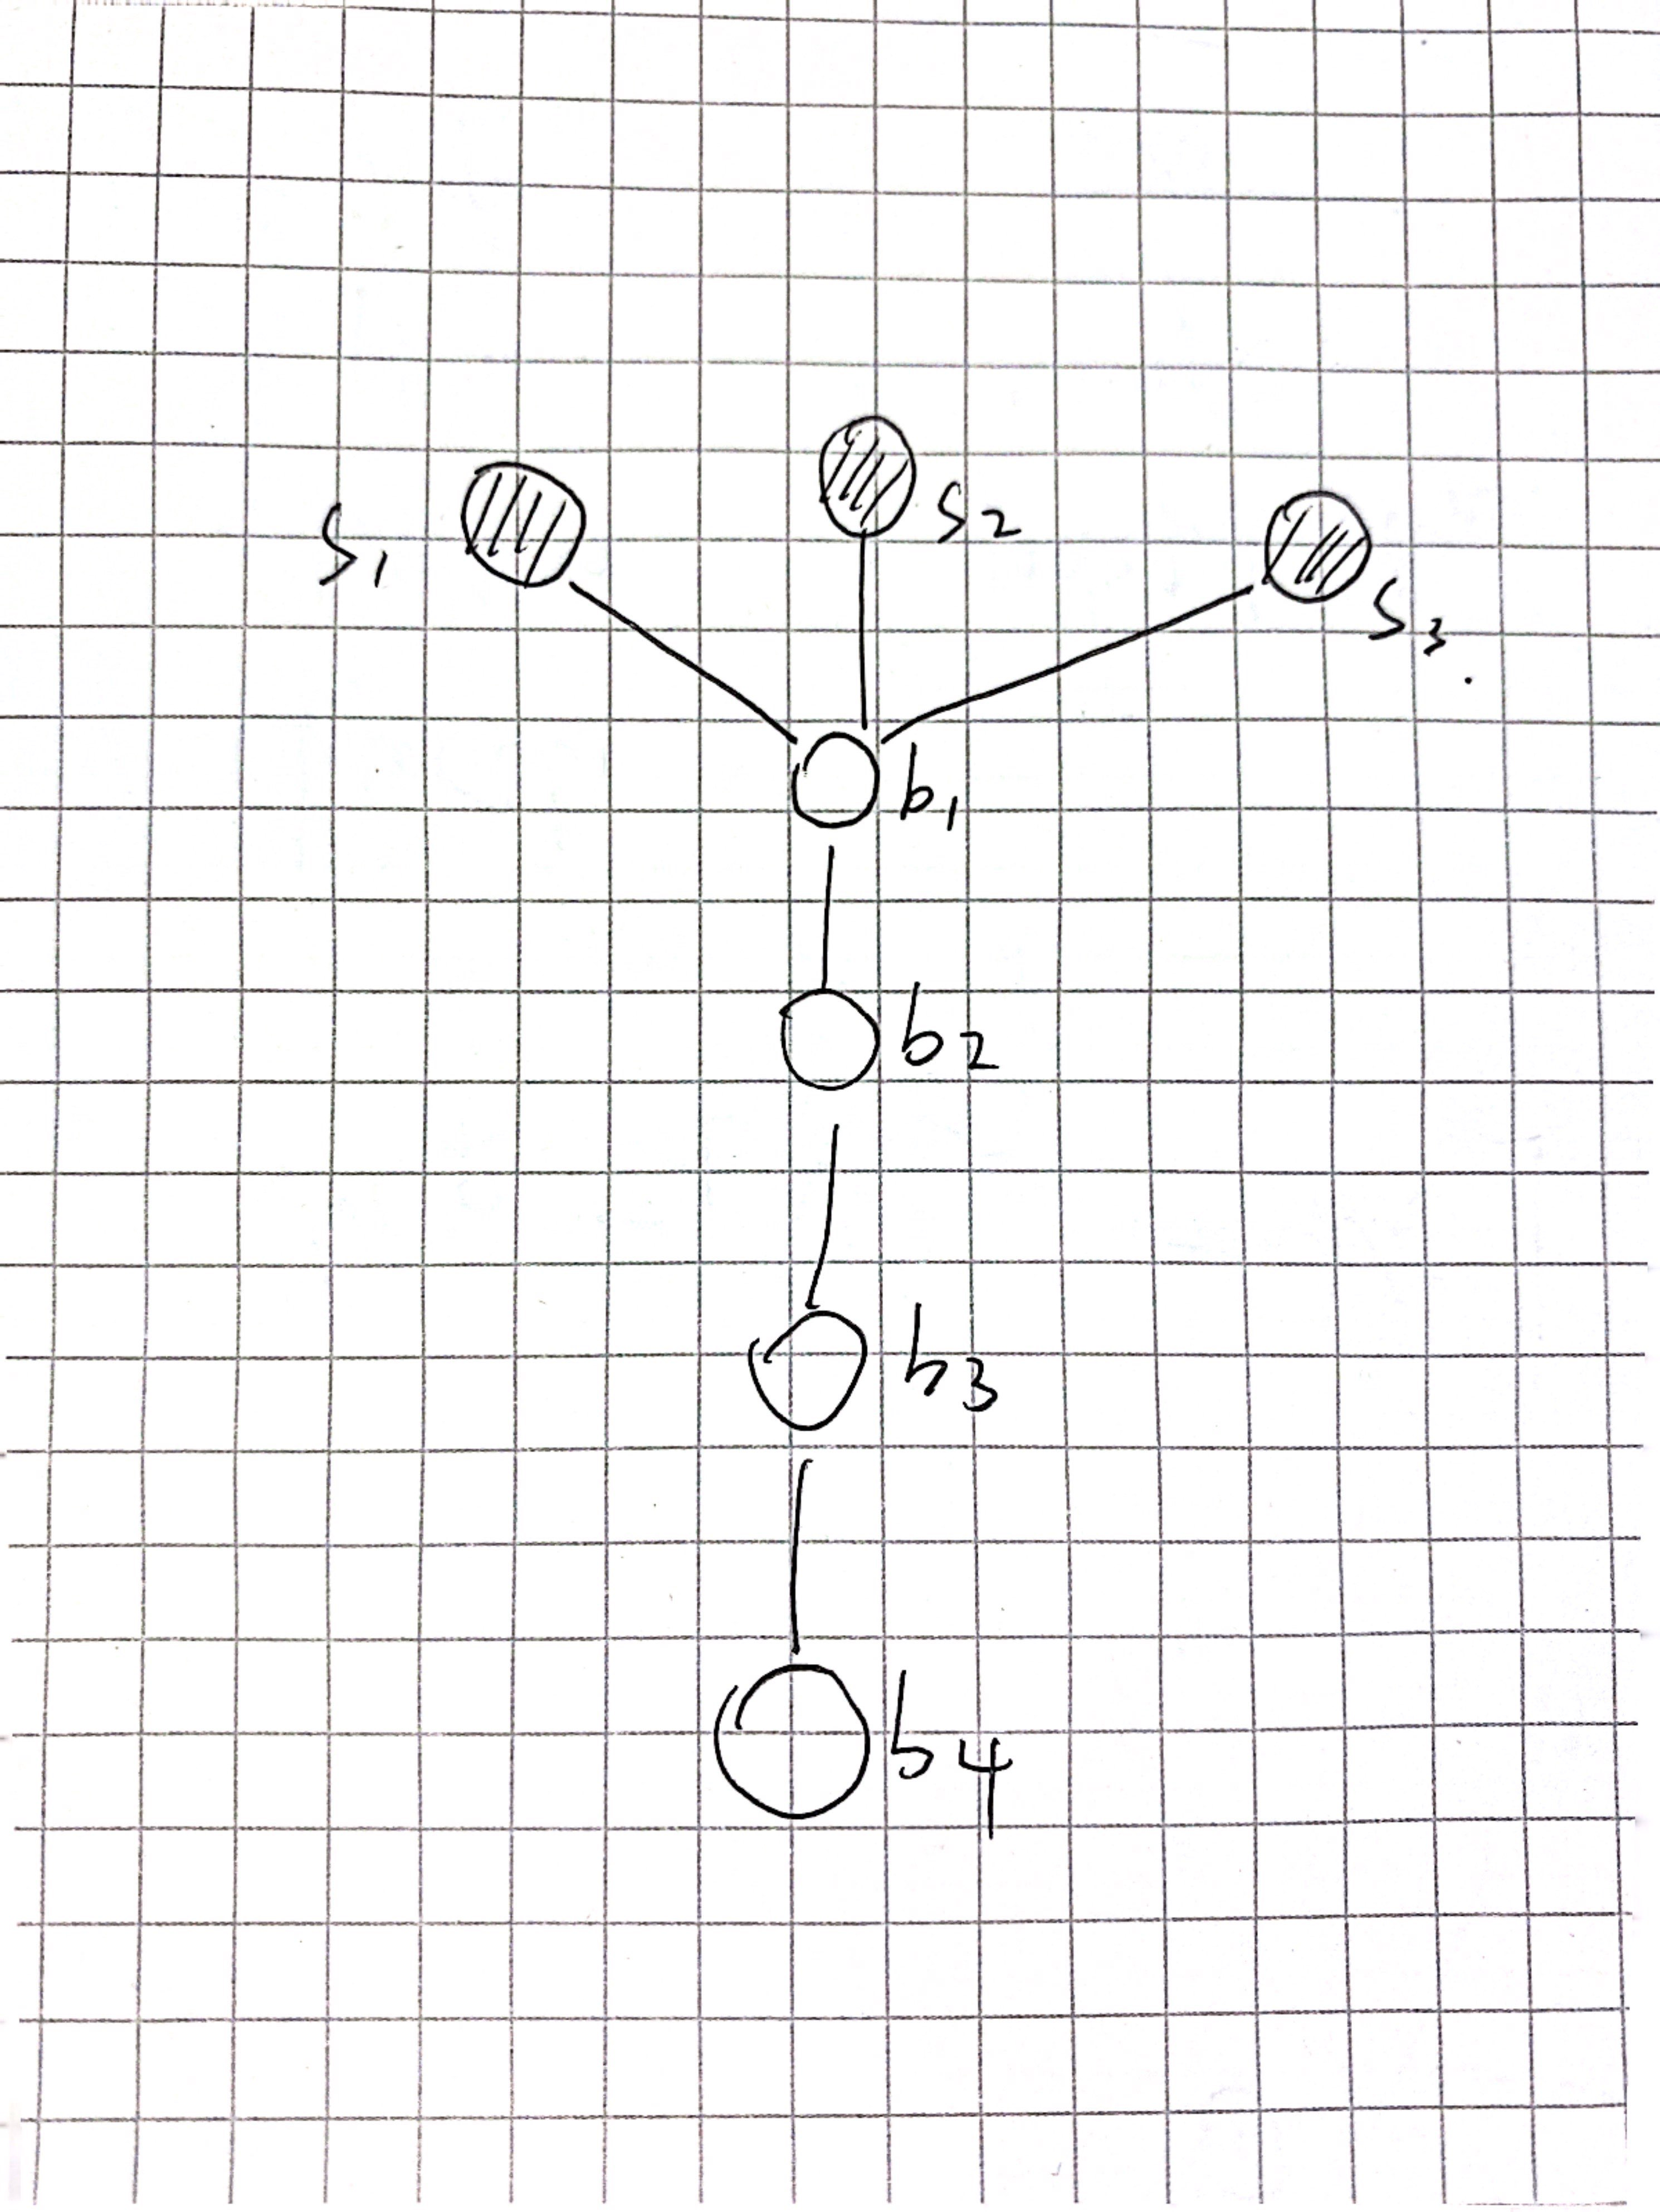
\includegraphics[width=0.6\textwidth]{./figure/DNA_counter_1.jpg}
  \caption{Network that can not be divided}
  \label{fig:DNACounter}
\end{figure}
\subsection{Multi-item Mechanism}
In a double auction scenario, we have multiple sellers, which means we also have multiple items. Therefore,
the multi-item mechanism may provide some valuable insights.\par
First, we try to adapt Generalized IDM(GIDM)\cite{GIDM} and Distance-based Network Auction mechanism for Multi-unit, Unit-demand buyers(DNA-MU)\cite{DNA-MU}.
However, these two methods are not IC. The counterexample is given in \ref*{fig:GIDMCounter}. The seller has
\(m = 4\) items. The example is from \cite{MUDAN-MUDAR}.
\begin{figure}[htbp]
  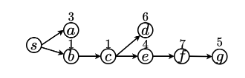
\includegraphics{./figure/GIDM_counter.png}
  \caption{Counter example for both GIDM and DNA-MU}
  \label{fig:GIDMCounter}
\end{figure}
\begin{itemize}
  \item \textbf{GIDM} If all player report truthfully. The winner will be \(b,c,d,e\)(Table \ref*{table:GIDMTruthful}).
        However, if \(f\) misreport her connection, then the allocation result will be \(a,b,c,f\)
        (Table \ref*{table:GIDMMisreport}).
        \begin{table}[htbp]
          \begin{tabular}{c|c|c|c}
            round & left items & winners         & \(\pi, p\)             \\
            \hline
            1     & 4          & \(\varnothing\) & \(\pi_b = 1, p_b = 0\) \\
            2     & 3          & \(\{b\}\)       & \(\pi_c = 1, p_c = 0\) \\
            3     & 2          & \(\{b,c\}\)     & \(\pi_d = 1, p_d = 5\) \\
            4     & 1          & \(\{b,c,d\}\)   & \(\pi_e = 1, p_e = 3\) \\
            \hline
          \end{tabular}
          \caption{GIDM with \(m = 4\). All buyer report truthfully\cite{MUDAN-MUDAR}}
          \label{table:GIDMTruthful}
        \end{table}
        \begin{table}[htbp]
          \begin{tabular}{c|c|c|c}
            round & left items & winners         & \(\pi, p\)             \\
            \hline
            1     & 4          & \(\varnothing\) & \(\pi_a = 1, p_b = 0\) \\
            2     & 3          & \(\{a\}\)       & \(\pi_b = 1, p_c = 0\) \\
            3     & 2          & \(\{a,b\}\)     & \(\pi_c = 1, p_d = 0\) \\
            4     & 1          & \(\{a,b,c\}\)   & \(\pi_f = 1, p_e = 6\) \\
            \hline
          \end{tabular}
          \caption{GIDM with \(m = 4\). \(f\) misreport connection \(r'_f = \varnothing\)\cite{MUDAN-MUDAR}}
          \label{table:GIDMMisreport}.
        \end{table}
  \item \textbf{DAN-MU} If all player report truthfully. The winner will be \(b,c,d,e\)
        (Table \ref*{table:DAN-MUTruthful}).
        However, if \(f\) misreport her connection, then the allocation result will be \(a,b,c,f\)(Table \ref*{table:DAM-MUMisreport}).
        \begin{table}[htbp]
          \begin{tabular}{c|c|c|c}
            round & left items & agent & \(\pi, p\)             \\
            \hline
            1     & 4          & \(b\) & \(\pi_b = 1, p_b = 0\) \\
            2     & 3          & \(c\) & \(\pi_c = 1, p_c = 0\) \\
            3     & 2          & \(d\) & \(\pi_d = 1, p_d = 5\) \\
            4     & 1          & \(e\) & \(\pi_e = 1, p_e = 3\) \\
            \hline
          \end{tabular}
          \caption{DAN-MU with \(m = 4\). All buyer report truthfully\cite{MUDAN-MUDAR}}
          \label{table:DAN-MUTruthful}
        \end{table}
        \begin{table}[htbp]
          \begin{tabular}{c|c|c|c}
            round & left items & agent & \(\pi, p\)             \\
            \hline
            1     & 4          & \(a\) & \(\pi_a = 1, p_b = 1\) \\
            2     & 3          & \(b\) & \(\pi_b = 1, p_c = 0\) \\
            3     & 2          & \(c\) & \(\pi_c = 1, p_d = 0\) \\
            4     & 1          & \(f\) & \(\pi_f = 1, p_e = 6\) \\
            \hline
          \end{tabular}
          \caption{DAN-MU with \(m = 4\). \(f\) misreport connection \(r'_f = \varnothing\)\cite{MUDAN-MUDAR}}
          \label{table:DAN-MUMisreport}.
        \end{table}
\end{itemize}
We can reduce our
problem to a multi-item problem if we connect several sellers to the same buyer with the same prices.
An example is shown in Fig \ref*{fig:MultiReduce}. It can be expected that the adapted method will not be IC either.\par
\begin{figure}[htbp]
  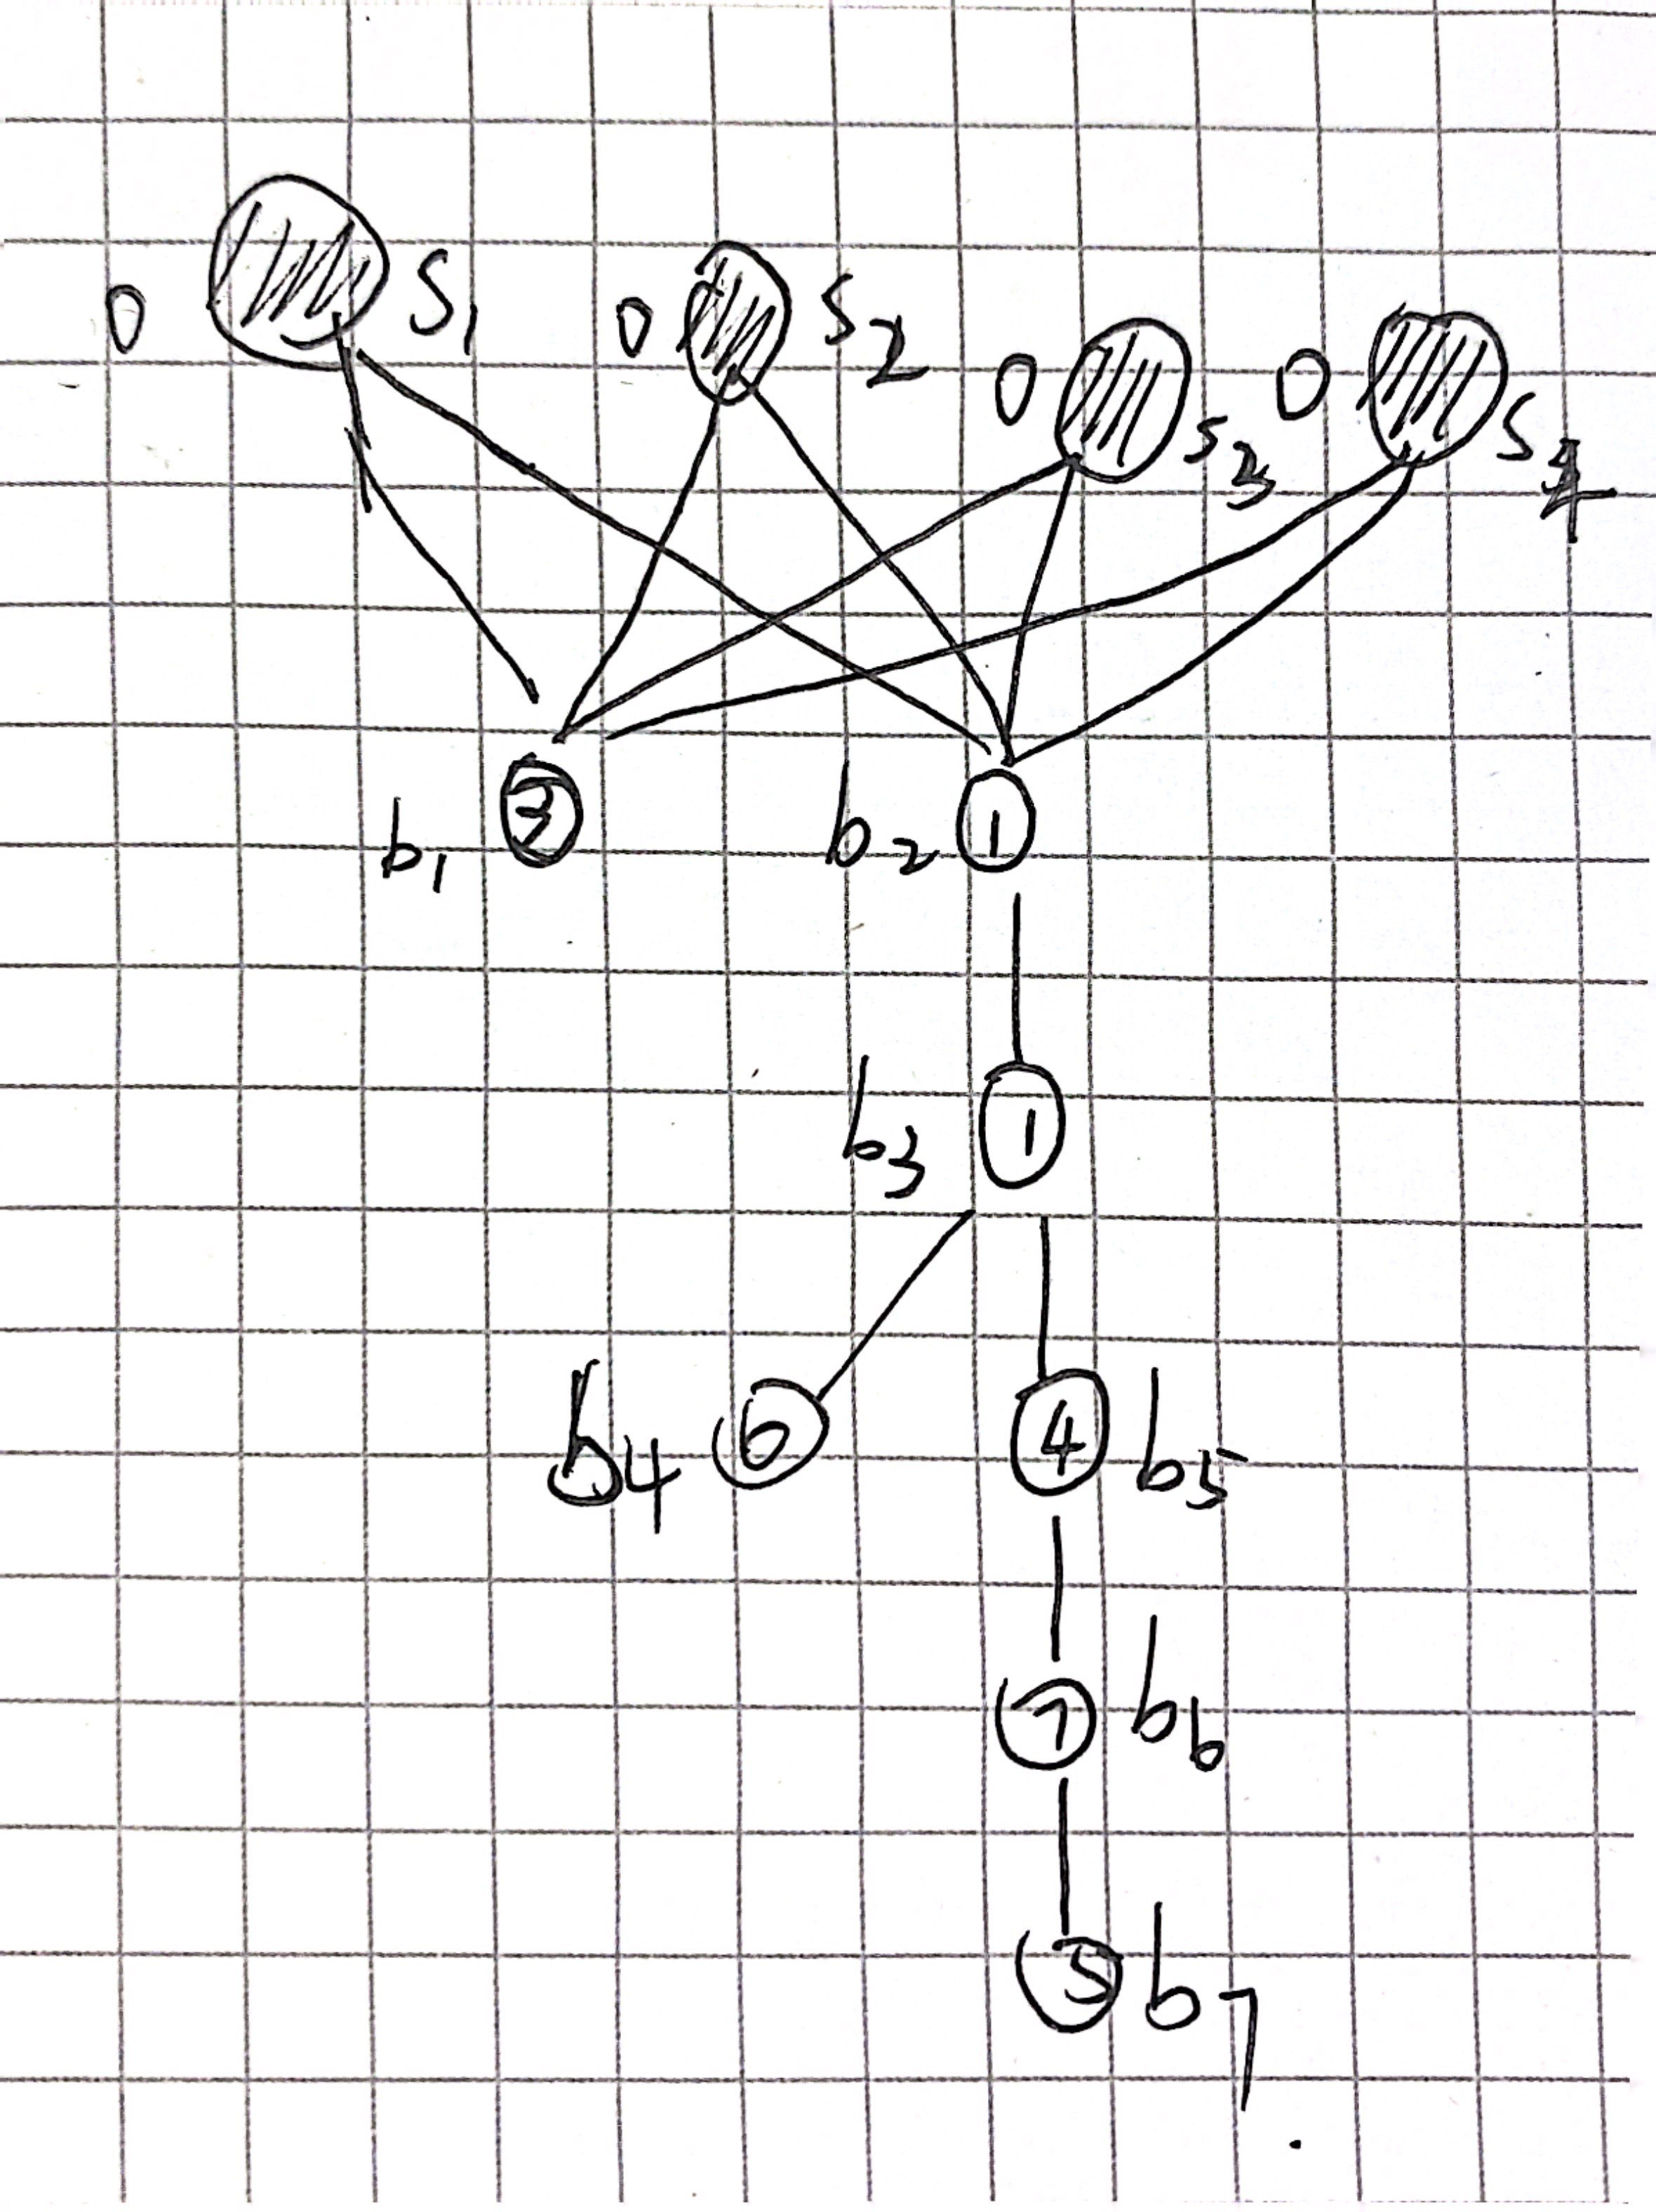
\includegraphics[width=0.6\textwidth]{figure/Multi_reduce.jpg}
  \caption{A reduction from multi-seller to multi-item}
  \label{fig:MultiReduce}

\end{figure}

We also look into two other IC mechanisms: MUDAN and LDM. These two methods are both layer-based mechanisms.
In our setting, items are held by different sellers. If the sellers are scattered around the network, the
network will degenerate into one layer since the children cannot get them, even if they may have higher
evaluations. An example is shown in Fig \ref*{fig:LayerDegenerate}.
\begin{figure}
  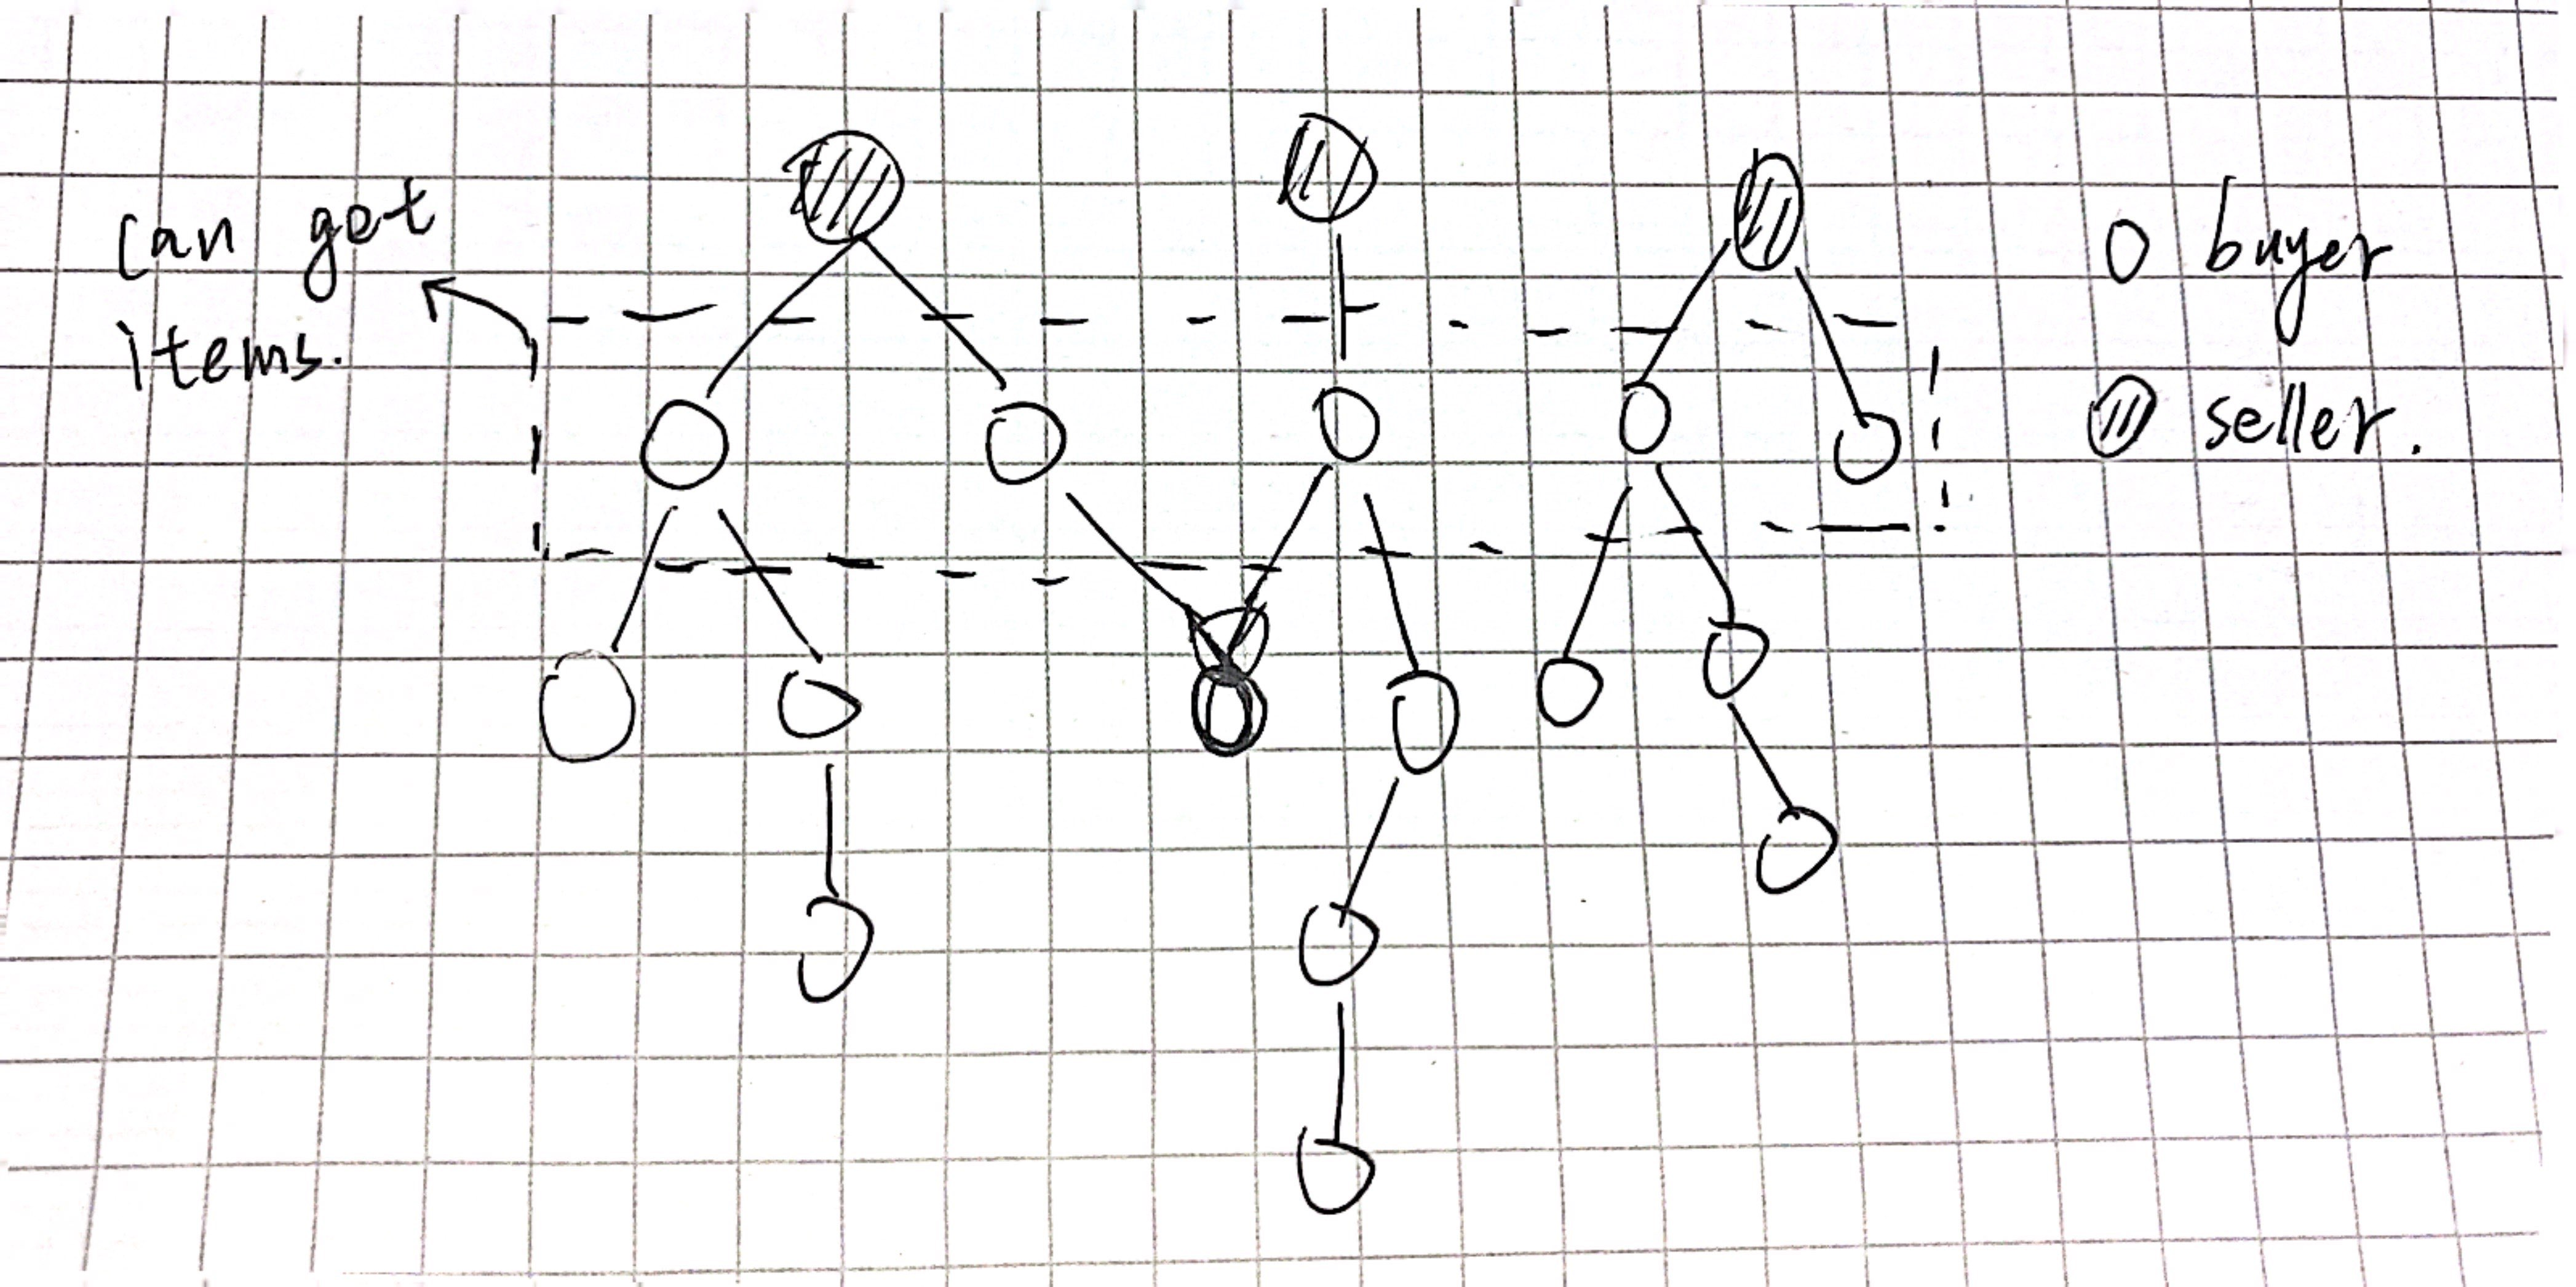
\includegraphics[width=0.6\textwidth]{./figure/Layer_degenerate.jpg}
  \caption{An example of the degeneration of a network to a single layer. }
  \label{fig:LayerDegenerate}
\end{figure}
\subsection*{Resale mechanism with leave and share}
In double-auction, we want people with high valuations to hold the item. Therefore, resale mechanisms are better than
layer-based mechanisms. Buyers with higher evaluations have more chances to get the item, while buyers with lower
evaluations are rewarded if they invite someone who gets it. From this insight, we designed a naive
resale mechanism that combined IDM with leave and share. The mechanism is described as follows,
\begin{enumerate}
  \item Sort the sellers in order of their price from lowest to highest.
  \item Let the seller with the lowest price sell the item using IDM. Other sellers are viewed as buyers with 0 valuations.
  \item The seller and the winner leave the network and share their connection.
  \item Repeat step 2, 3 until no seller can sell the item.
\end{enumerate}
However, this mechanism is not IC since the seller with a lower price has more chance to sell their
item at a high price, and the seller has the incentive to misreport a lower price. In the following example, if \(s_1\)
\(s_2\) both report truthfully (Fig \ref*{fig:LeaveTruthful}), then \(s_2\) will receive \(9\). But
if he misreport \(2\), he will receive \(10\)(Fig \ref*{fig:LeaveMisreport}). Therefore, he has the incentive to misreport.
\begin{figure}[htbp]
  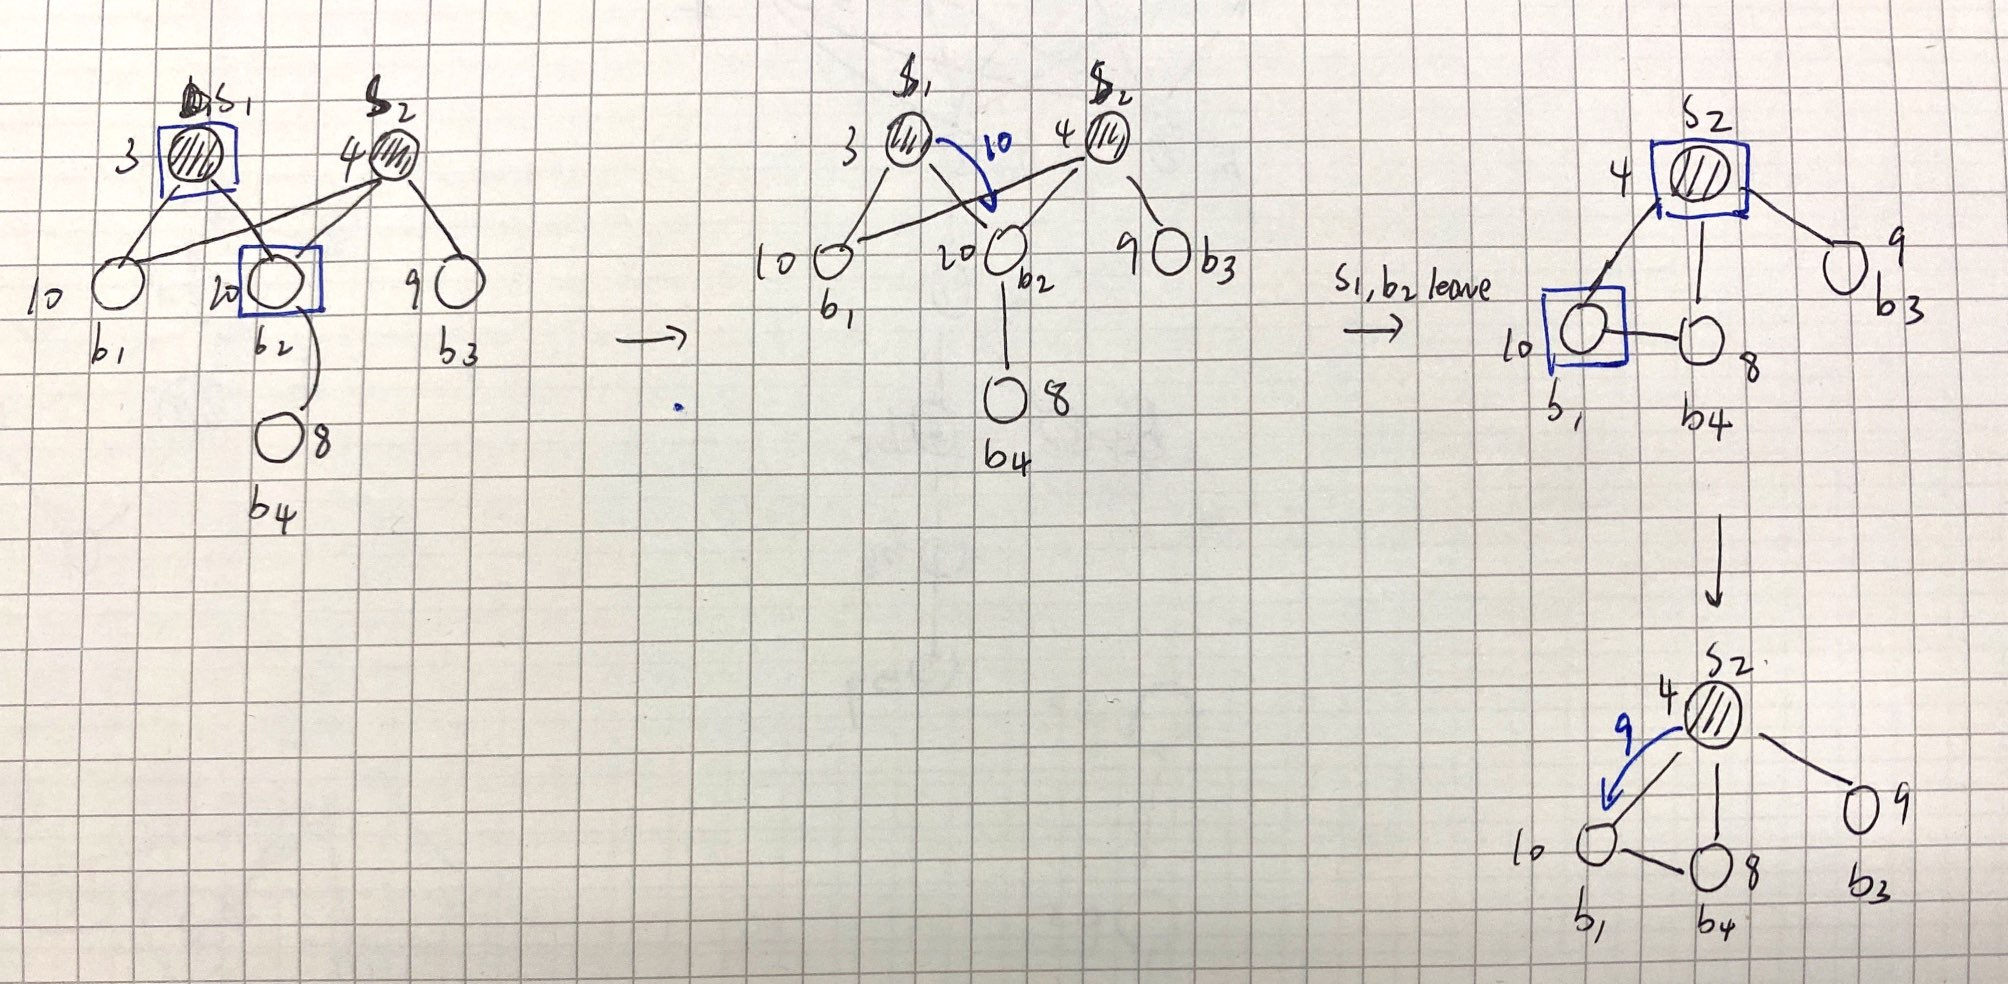
\includegraphics[width=0.6\textwidth]{figure/Leave_truthful.jpg}
  \caption{A run of the naive algorithm. All player report truthfully}
  \label{fig:LeaveTruthful}
\end{figure}
\begin{figure}[htbp]
  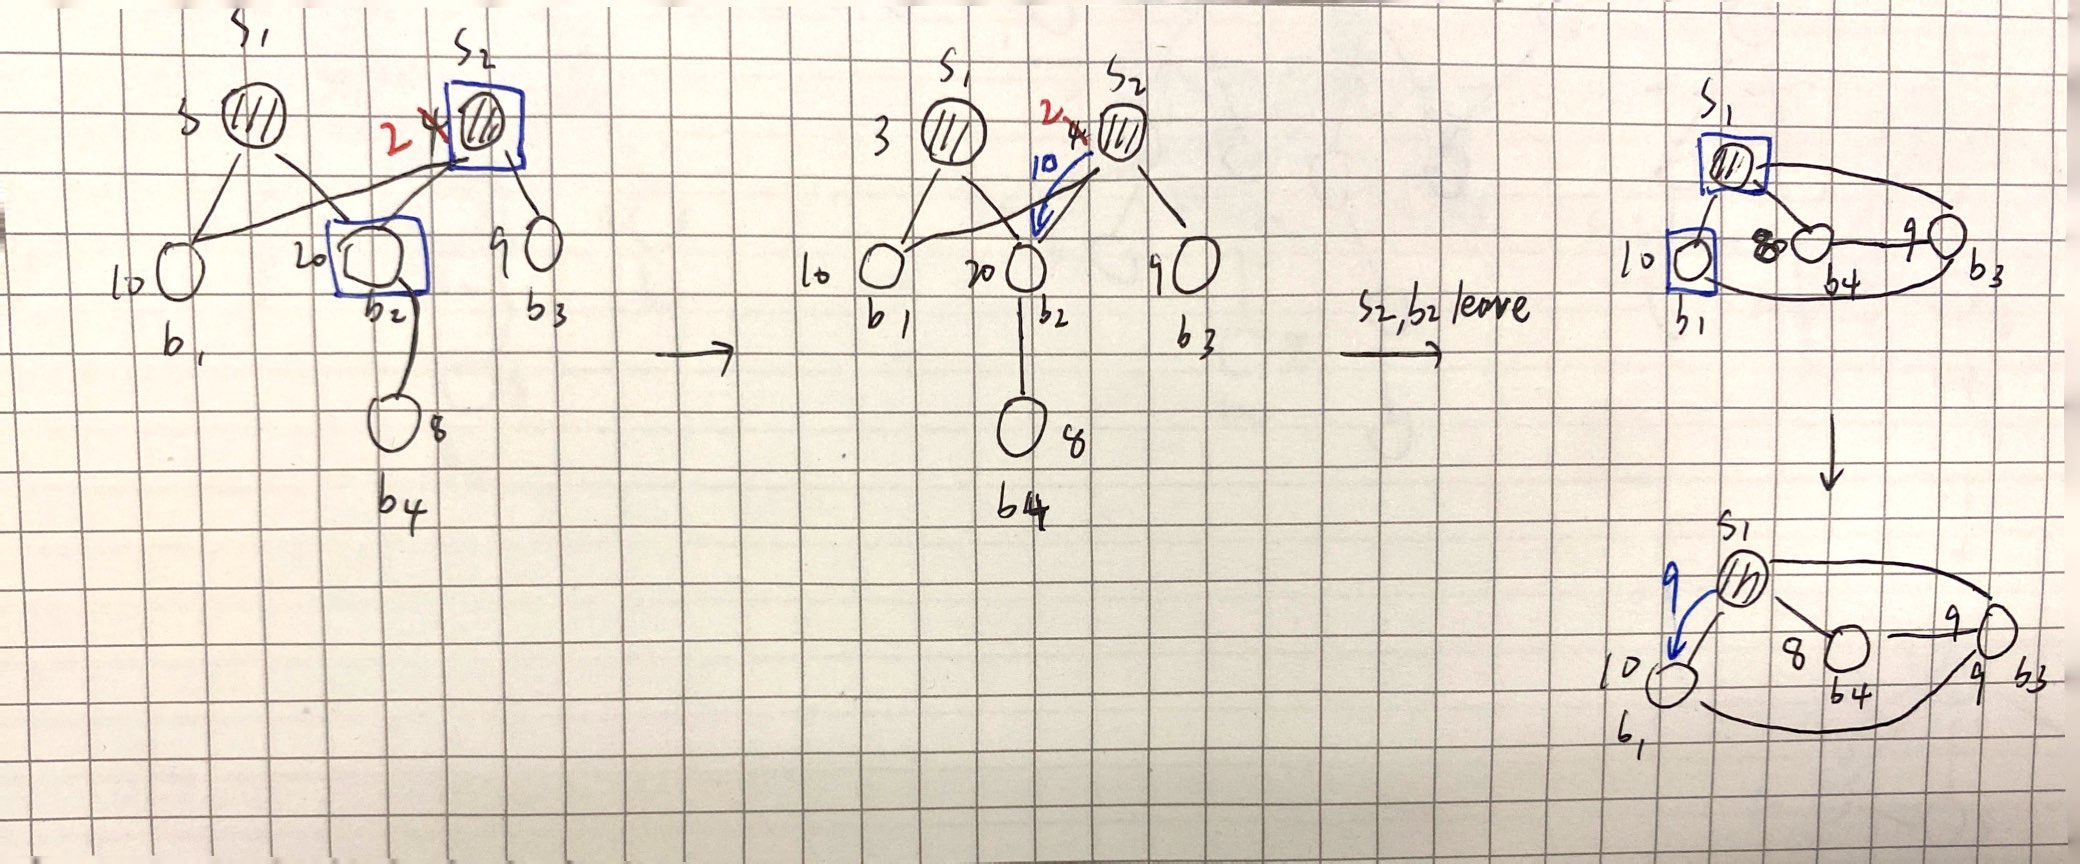
\includegraphics[width=0.6\textwidth]{figure/Leave_misreport.jpg}
  \caption{A run of the naive algorithm. \(s_2\) misreport \(2\)}
  \label{fig:LeaveMisreport}
\end{figure}

\subsection*{Resale with leave and share, eliminating highest \(m\) bid}
Then we modified the original algorithm. The main idea is still the same, but when calculating
the price using IDM, we first eliminate the highest \(m\) bids, where \(m\) is the number of unmatched sellers.
As a result, the seller cannot profit more by misreporting, and neither can the buyer. However, we still have to do
more work to show and prove that this mechanism is IC.
Moreover, Since we have eliminated the highest bids, some deals that might have worked will fail.
However, this will not be a problem if the network is big enough and the number of the buyer is much greater than the seller.